%!TEX root = ../report.tex


\chapter{Implementation and Validation}
\label{chap:chap4}

\section*{}

In this chapter, further details about the prototype's main features and the methodologies used when developing the prototype, as well as in the the validation process, will be explored.

The Implementation section will go into details about the processes used to maintain a sane development environment by taking advantage of several tools that automated most of the common tasks. The main implemented features will also be analysed.

By this point, the validation of the prototype will be analysed, by explaining the performed user tests, as well the analysis of the results.


\section{Implementation} % (fold)
\label{sec:implementation}

    
  \subsection{Technologies used} % (fold)
  \label{sub:technologies}

    The following technologies were used during the development of the application.

    \subsubsection{Git} % (fold)
    \label{ssub:git}
    
    The chosen version control system to manage the source code was git\footnote{git: \url{http://git-scm.com}}. \\
    The use of branches\footnote{git branches: \url{http://git-scm.com/book/en/Git-Branching-What-a-Branch-Is}} and tags\footnote{git tags: \url{http://git-scm.com/book/en/Git-Basics-Tagging}} allowed for a sane code development environment, e.g., marking release commits or working on experimental features.

    % subsubsection git (end)

    \subsubsection{Spotify Desktop Client} % (fold)
    \label{ssub:subsection_name}
      Spotify Applications are developed in its runtime environment - the Spotify Desktop Client.

      To open a Spotify Application, locally, one writes the following in the search bar: spotify:app:rama

      Where \emph{rama} is the application identifier declared in the \emph{manifest.json} file\footnote{file located at the root of the project folder}.

      Example:

      \lstinputlisting[caption={manifest.json: \emph{BundleIdentifier} is the application's identifier; \emph{Dependencies} declares the Application's API dependencies.}, style=htmlcssjs]{snippets/manifest.json}

      There are useful options for development located in the "Develop" tab (\ref{fig:html5_support}).
      The "Show Inspector" option opens the \emph{Webkit Development Tools} (\ref{ssub:webkit_tools}) window.

      \begin{figure}
        \begin{center}
          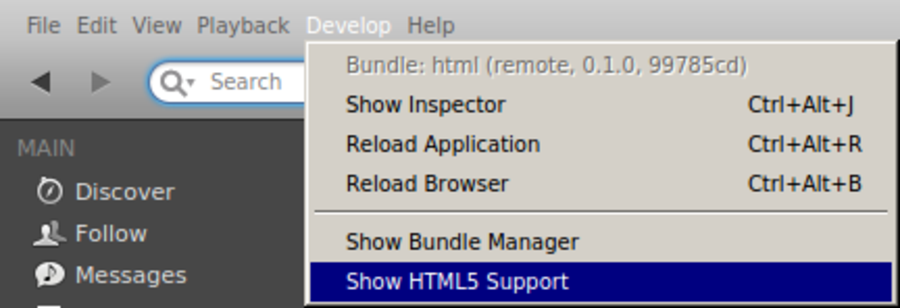
\includegraphics[width=0.8\textwidth]{html5_support.pdf}
        \end{center}
        \caption{\emph{Develop} Tab}
        \label{fig:html5_support}
      \end{figure}
    
    \subsubsection{Webkit Development Tools - webkit.org} % (fold)
    \label{ssub:webkit_tools}

      The webkit tools provides a bundle of tools for web development.

      \begin{figure}
        \begin{center}
          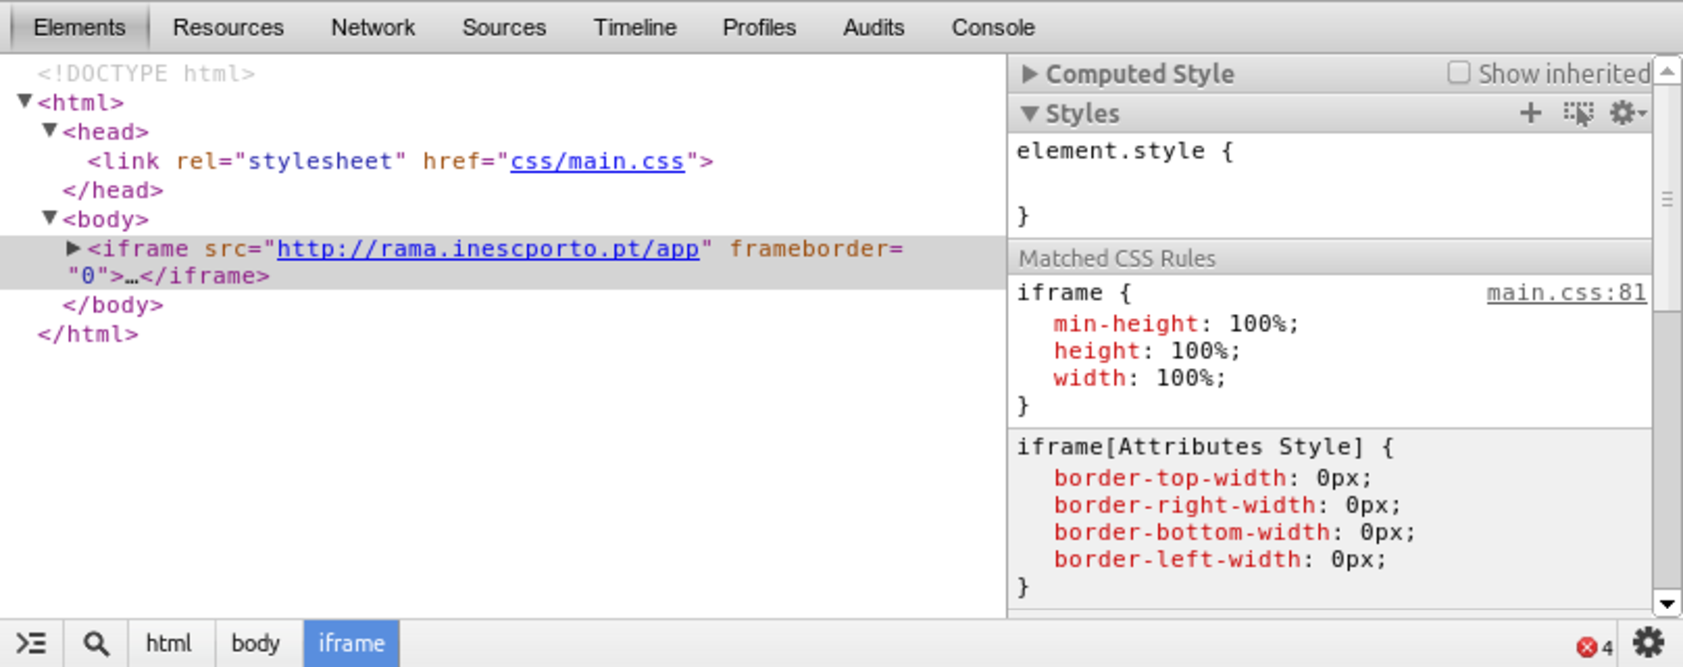
\includegraphics[width=\textwidth]{webkit_inspector.pdf}
        \end{center}
        \caption{Webkit: \emph{Inspector} tab view. Other tools available: \emph{Resources, Network, Sources, Timeline, Profiles, Audits} and \emph{Console}.}

        \label{fig:webkit_inspector}
      \end{figure}

      Being the most important:

      \begin{description}
        \item[Inspector] Allows to inspect the resulting Html and CSS and edit the code and see the application automatically reflect those changes (\ref{fig:webkit_inspector}).
        \item[Network] Shows a timeline list of resources that where loaded from external sources (sometimes local) (\ref{fig:webkit_network}).
        \item[Profile] Allows to identify which parts of the javascript code are being executed frequently, and which ones might be creating a performance issue (\ref{fig:webkit_profile}).
        \item[Audit] Helps to understand which CSS rules are not being used (\ref{fig:webkit_audit}).
        \item[Console] Javascript interpreter that also works as the log output for the application (\ref{fig:webkit_console}).

      \end{description}

      \begin{figure}
        \begin{center}
          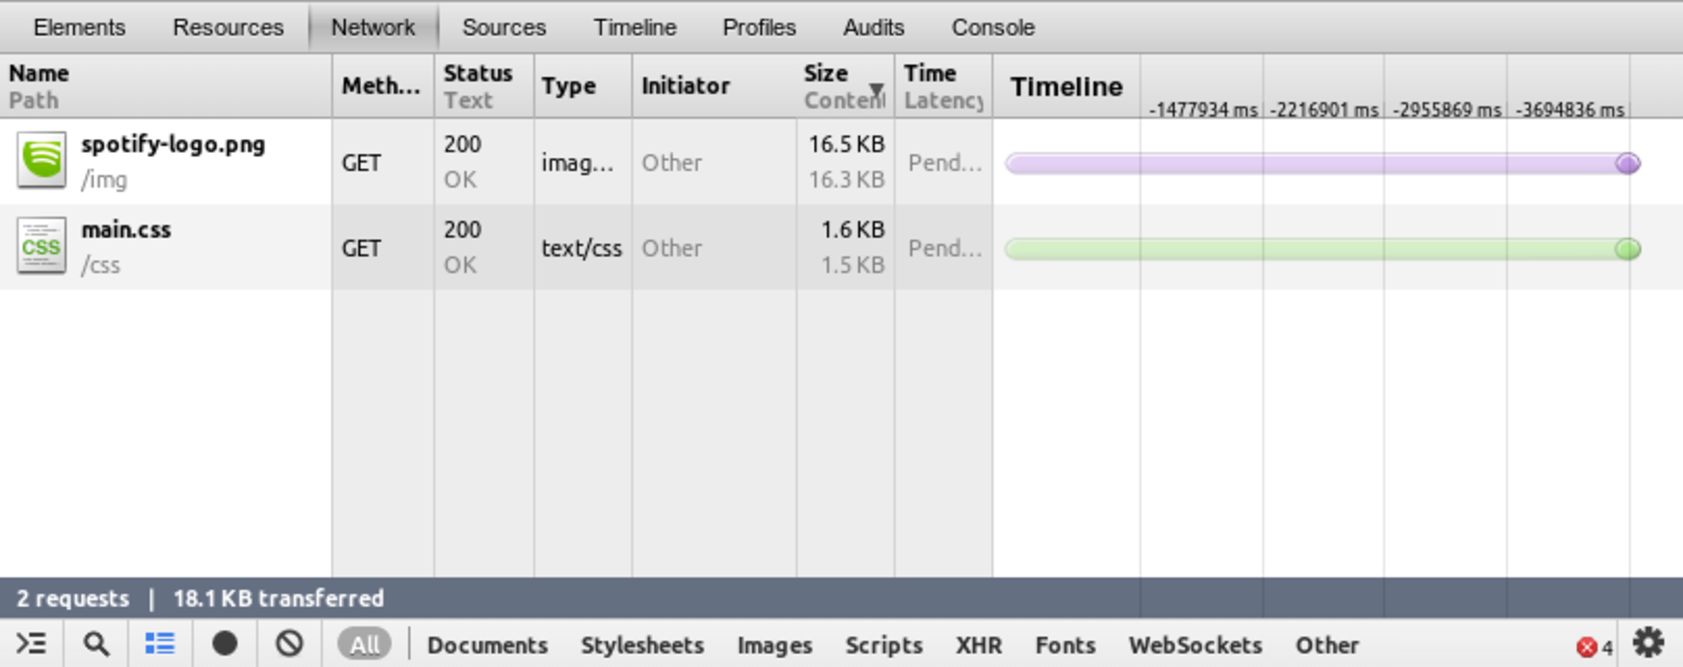
\includegraphics[width=\textwidth]{webkit_network.pdf}
        \end{center}
        \caption{Webkit Network}
        \label{fig:webkit_network}
      \end{figure}

      \begin{figure}
        \begin{center}
          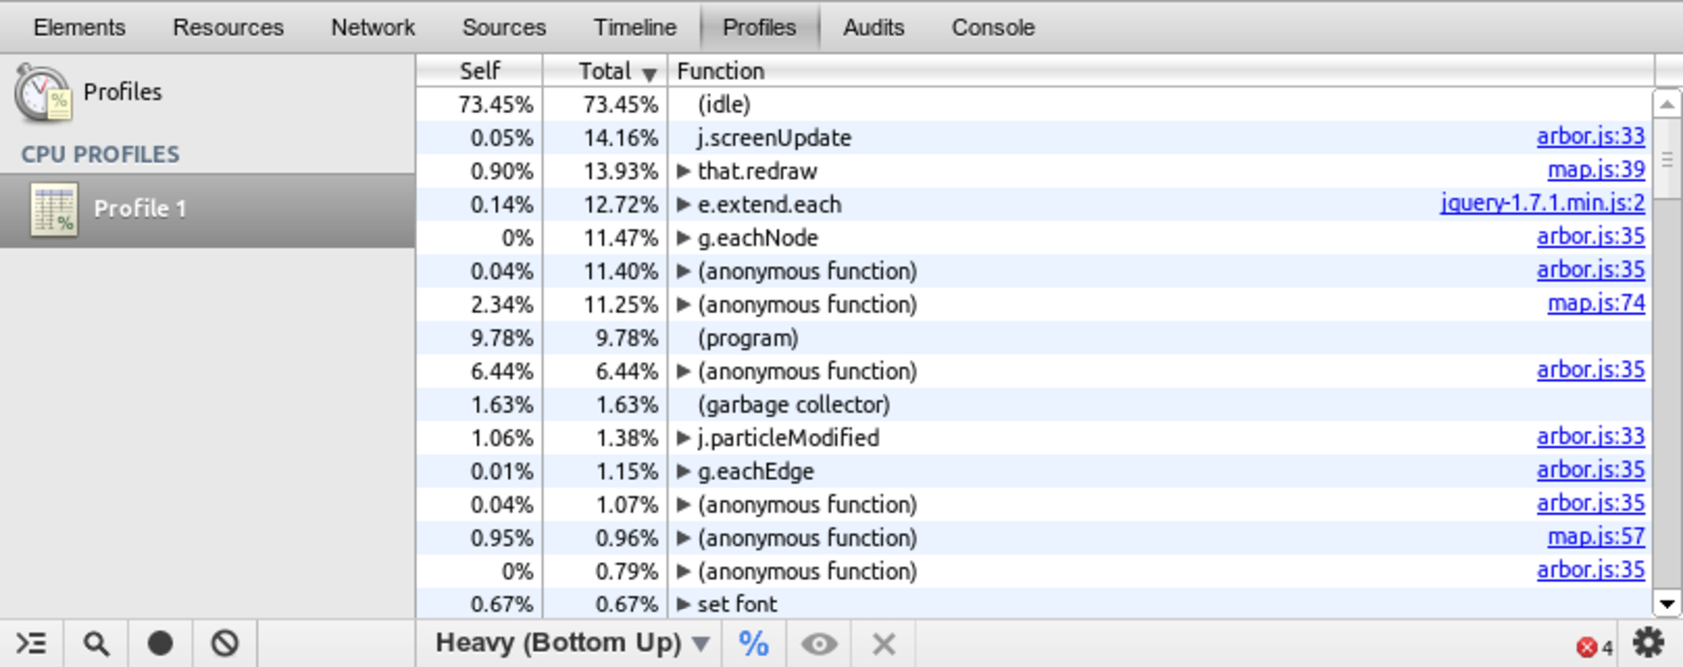
\includegraphics[width=\textwidth]{webkit_profile.pdf}
        \end{center}
        \caption{Webkit Profile: Canvas render functions are the ones taking up most of the processing cycles. However there is a JQuery function that used 12.75\% of processing time, which might indicate a performance issue to be improved.}
        \label{fig:webkit_profile}
      \end{figure}

      \begin{figure}
        \begin{center}
          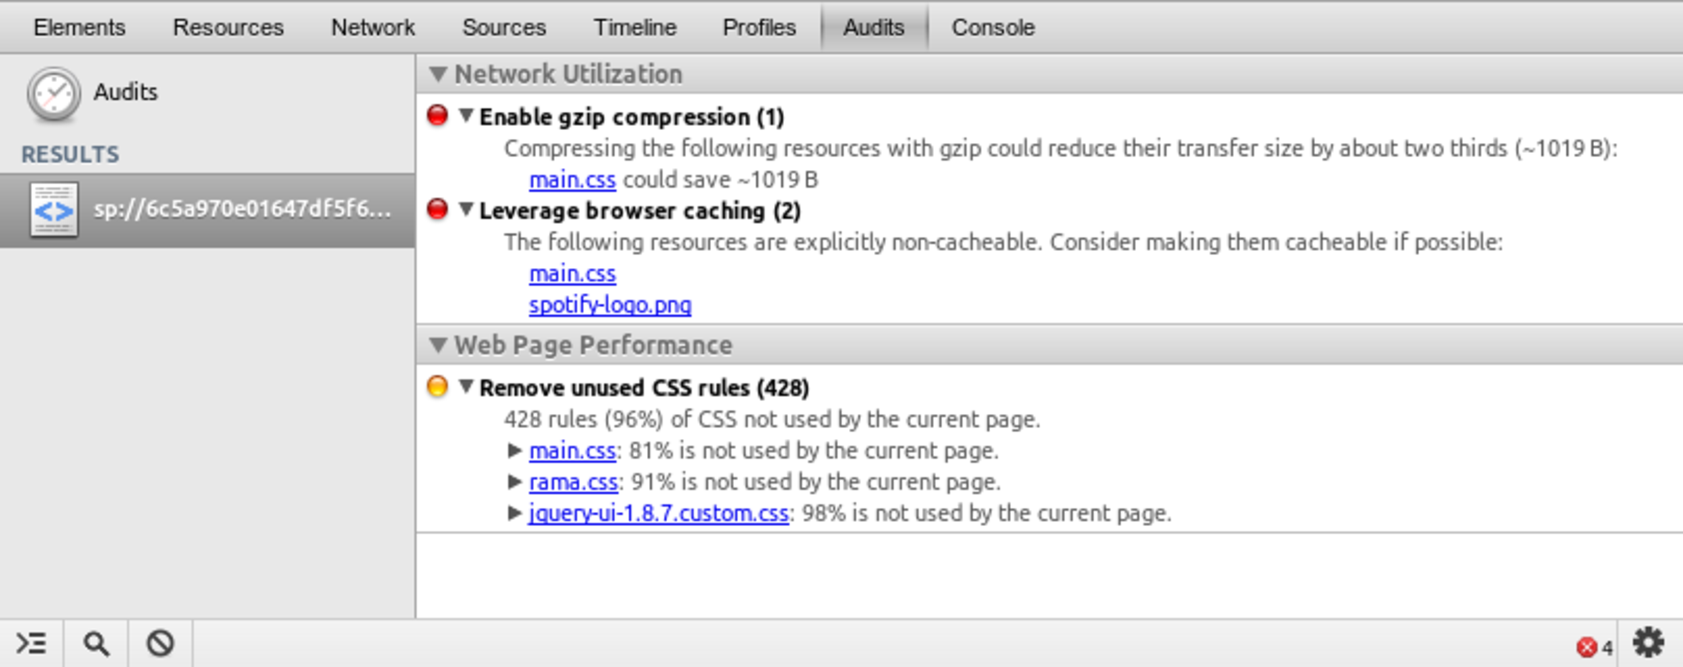
\includegraphics[width=\textwidth]{webkit_audit.pdf}
        \end{center}
        \caption{Webkit Audit: 96\% of the CSS code is not being used indicates a issue to be solved.}
        \label{fig:webkit_audit}
      \end{figure}

      \begin{figure}
        \begin{center}
          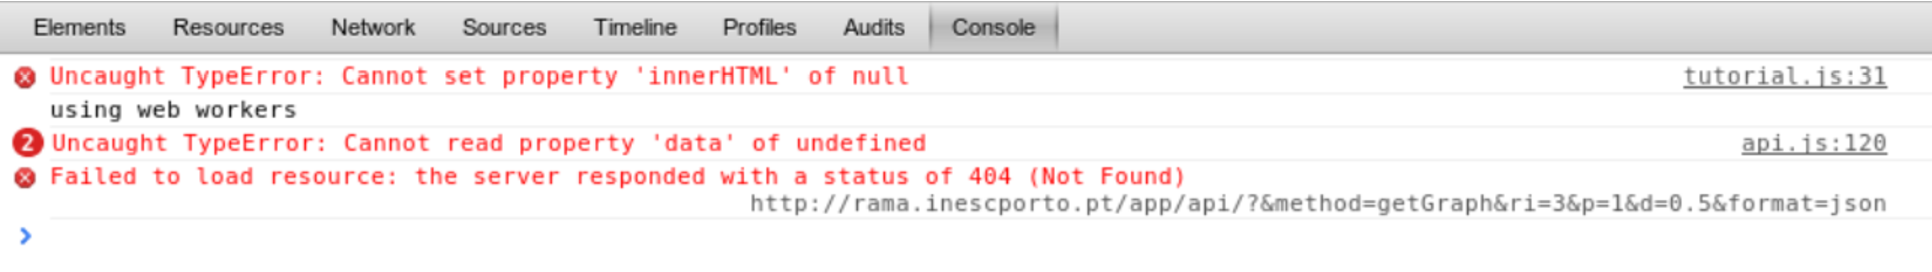
\includegraphics[width=\textwidth]{webkit_console.pdf}
        \end{center}
        \caption{Webkit Console: Javascript errors are reported there (and highlighted in red as well).}
        \label{fig:webkit_console}
      \end{figure}

    \subsubsection{Gruntjs - gruntjs.com} % (fold)
      \label{ssub:gruntjs}
        Gruntjs is a Javascript task runner.
        It allows to automate most of the repetitive tasks when developing a website.
        Very useful for testing, compiling and code optimization.

    \subsubsection{Npmjs - npmjs.org} % (fold)
    \label{ssub:npm}
      Package dependency manager for nodejs - Node Packaged Modules.
      Node packages will be used, since Gruntjs plugins are all nodejs packages (as well as Grunt itself).

      A npm configuration file (\emph{package.json}) allows to identify the packages that the application depends upon, as well as its versions.

      Example: 

      \lstinputlisting[caption={\emph{package.json}: "*" means that npm should always install the latest version of that package.}, style=htmlcssjs]{snippets/package.json}

      Note that these software packages are for development only. Not needed at all when running production code.

    \subsubsection{Bower - bower.io} % (fold)
    \label{ssub:bower}
    
    Bower is also a package manager, but oriented for web front-end packages.
    It mainly supports runtime software packages, which are needed for production code.

    % subsection bower (end)

    \subsubsection{vis.js - visjs.org} % (fold)
    \label{ssub:visjs}
      Javascript framework for visualization.
      It provides a few visual components, including graphs.


  \subsection{Implemented Features} % (fold)
    \label{sub:main_features}
    
    The requirements for the prototype are as following:

    \begin{itemize}
      \item Visualization of relations between artists by means of a visual tool;
      \item Edition of the visualization using several parameters;
      \item Edition of the graph by allowing to remove and add new nodes;
      \item Visualize tags/genres (that describe an artist) in the graph representation.
    \end{itemize}

    All of these were implemented.

    \subsubsection{Visulization of the Artists Map} % (fold)
      \label{ssub:visualization}
    
      The application automatically draws the map with the current playing artist as the main node, as seen in Figure~\ref{fig:graph_rootnode}.

      \begin{figure}[tb]
        \begin{center}
          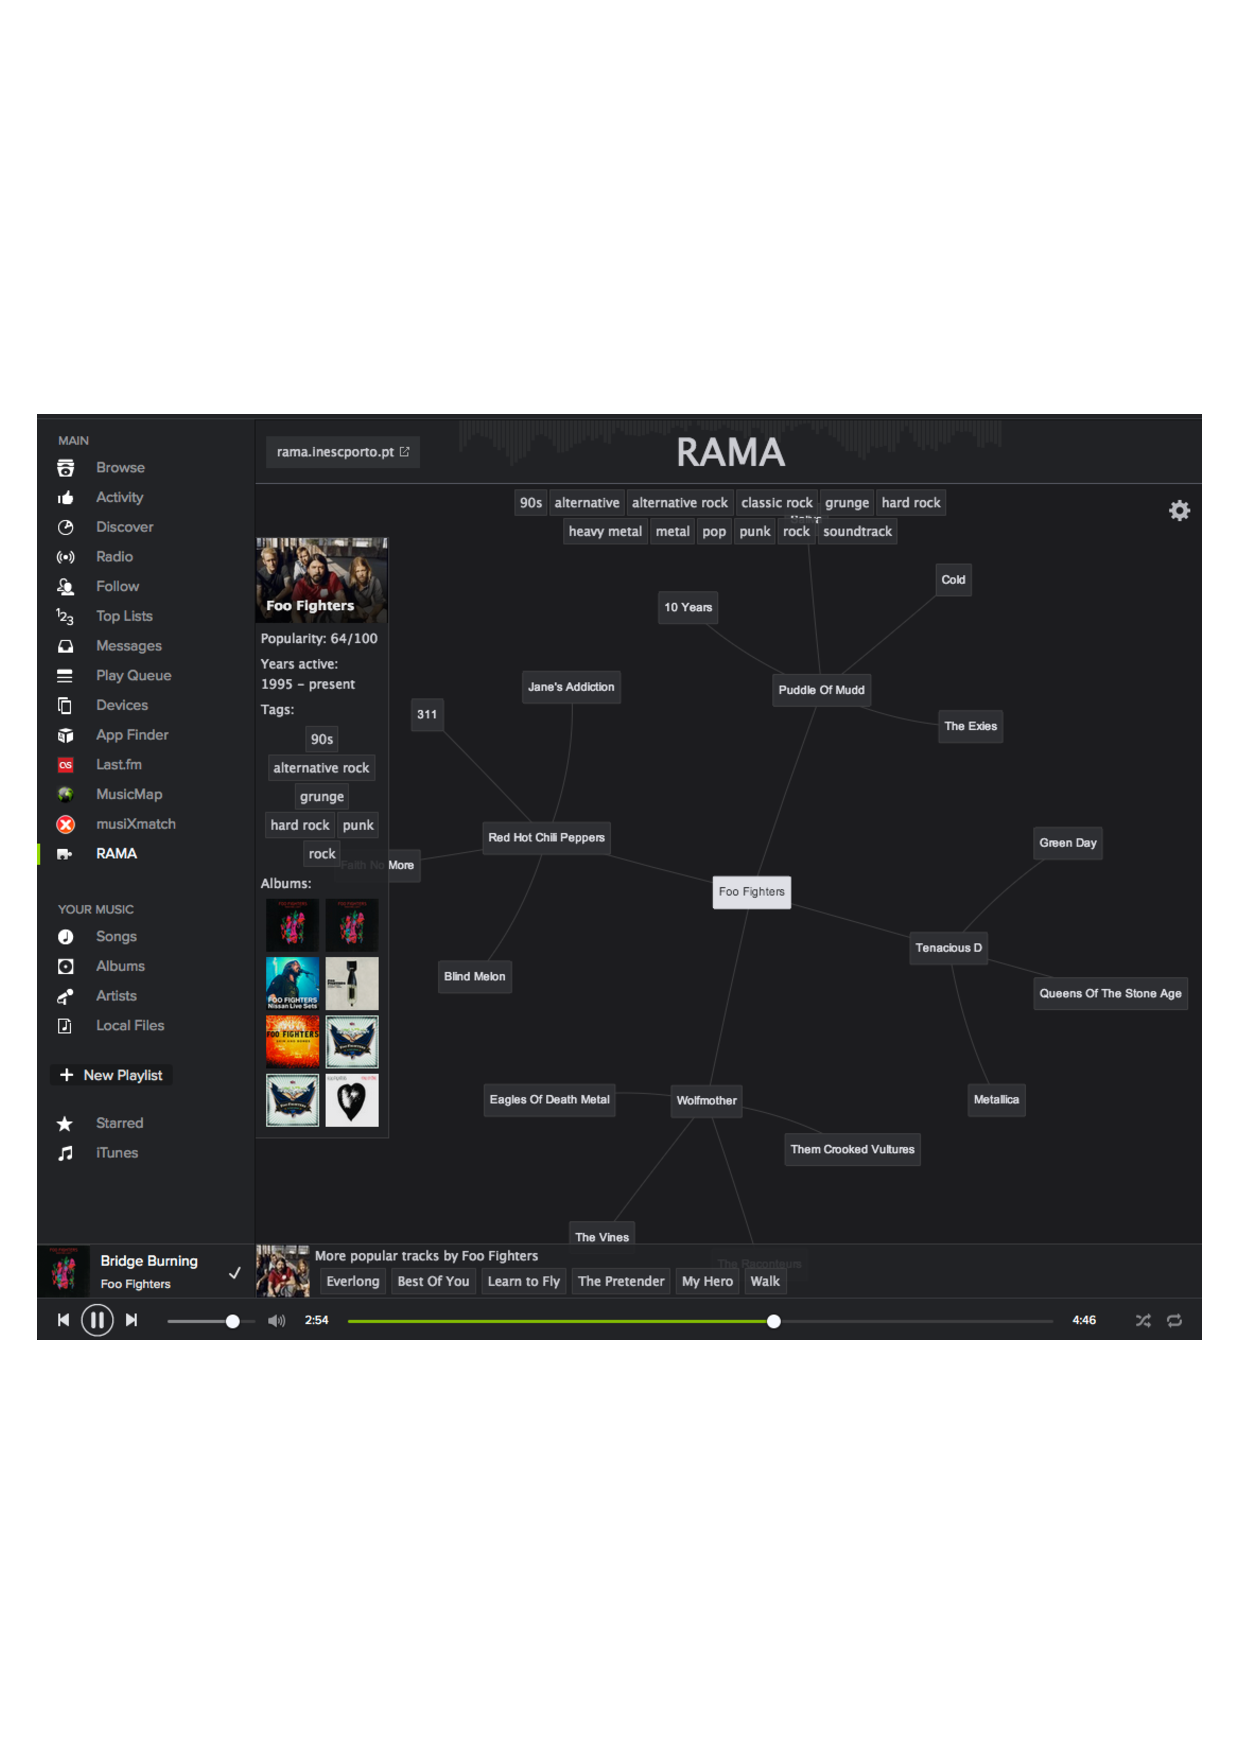
\includegraphics[width=\textwidth]{graph_rootnode.pdf}
        \end{center}
        \caption{The first drawn graph uses the current playing artist (lower left corner) as the root node.}
        \label{fig:graph_rootnode}
      \end{figure}

      The graph-like structure is created by recursively fetching a list of related artists from each artist. Once a certain pre-established limit of recursive levels is reached\footnote{depth value of a graph}, the algorithm stops.

      The graph creation algorithm is as follows:

      % change the code the attachments
      \lstinputlisting[
        caption={Simplified graph creation algorithm in Javascript (duplicate nodes checking is encapsulated in the insertNode function)}, style=htmlcssjs
      ]
      {snippets/map_creation_alg.js}

      The maximum number of nodes that the graph might have, can be calculated like so:

      \begin{equation}
          \sum_{i=0}^{d} b ^ i
      \end{equation}

      Given $d$ to be the depth value and $b$ the branching value of the graph.

      This algorithm, albeit simplified, represents the basic flow when constructing a graph, or more specifically, a tree.
      Since that, in this case of study, the direction of the edges of the graph is not relevant in any way to the artists' map, all of the edges are considered to be undirected.

      Assuming that the insertNode() function checks for duplicate nodes, i.e., it only inserts unique nodes into the graph, then the resulting graph is one of a tree, since there are no simple cycles in the graph.
      An example of this behaviour can be seen in Figure~\ref{fig:graph_treemode}.

      \begin{figure}[tb]
        \begin{center}
          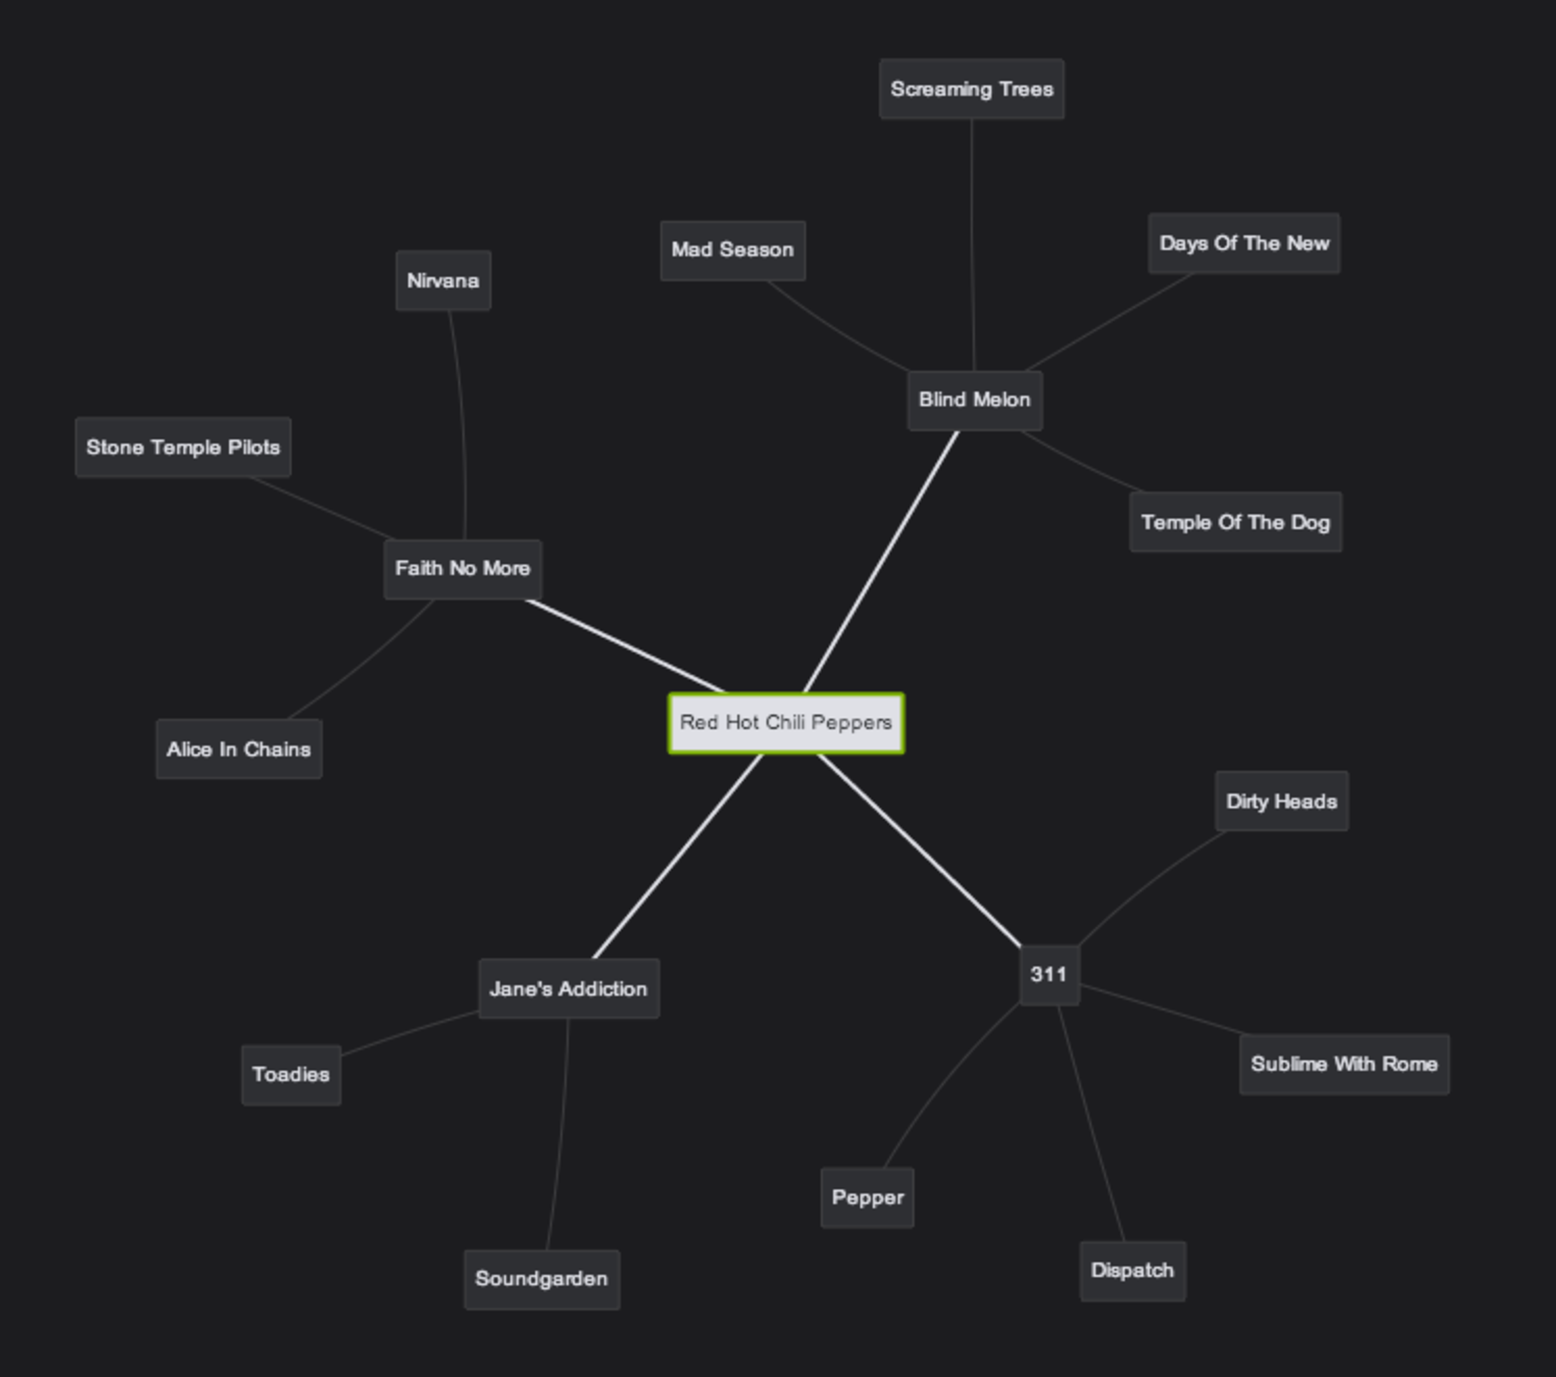
\includegraphics[width=\textwidth]{map_creation_treemode.pdf}
        \end{center}
        \caption{Graph created like a tree with "Red Hot Chilli Peppers" as the root node.}
        \label{fig:graph_treemode}
      \end{figure}

      This approach, however, is not showing all of the available information.
      Given this same example (Figure~\ref{fig:graph_treemode}), the artist node "Stone Temple Pilots" is a child of the node artist "Faith No More".
      The algorithm inserted the latter first into the graph.
      After that, when retrieving the childs of "Jane's Addiction", "Stone Templo Pilots" is contained in that list, and so the insertNode() function discards the node since it is a duplicate.
      But that means that there is a connection between the both of them that is being discarded.

      \paragraph{Graph's Tree Mode} \hfill \\
      To build a graph with all the connections that exist between all of the artists in the graph, the insertNode() function would need to insert the missing edge into the graph by analysing the current graph state.
      This method creates a graph by definition, while the previous one created a tree graph.
      An example of this behaviour can be seen in Figure~\ref{fig:graph_notreemode}.
      \begin{figure}[tb]
        \begin{center}
          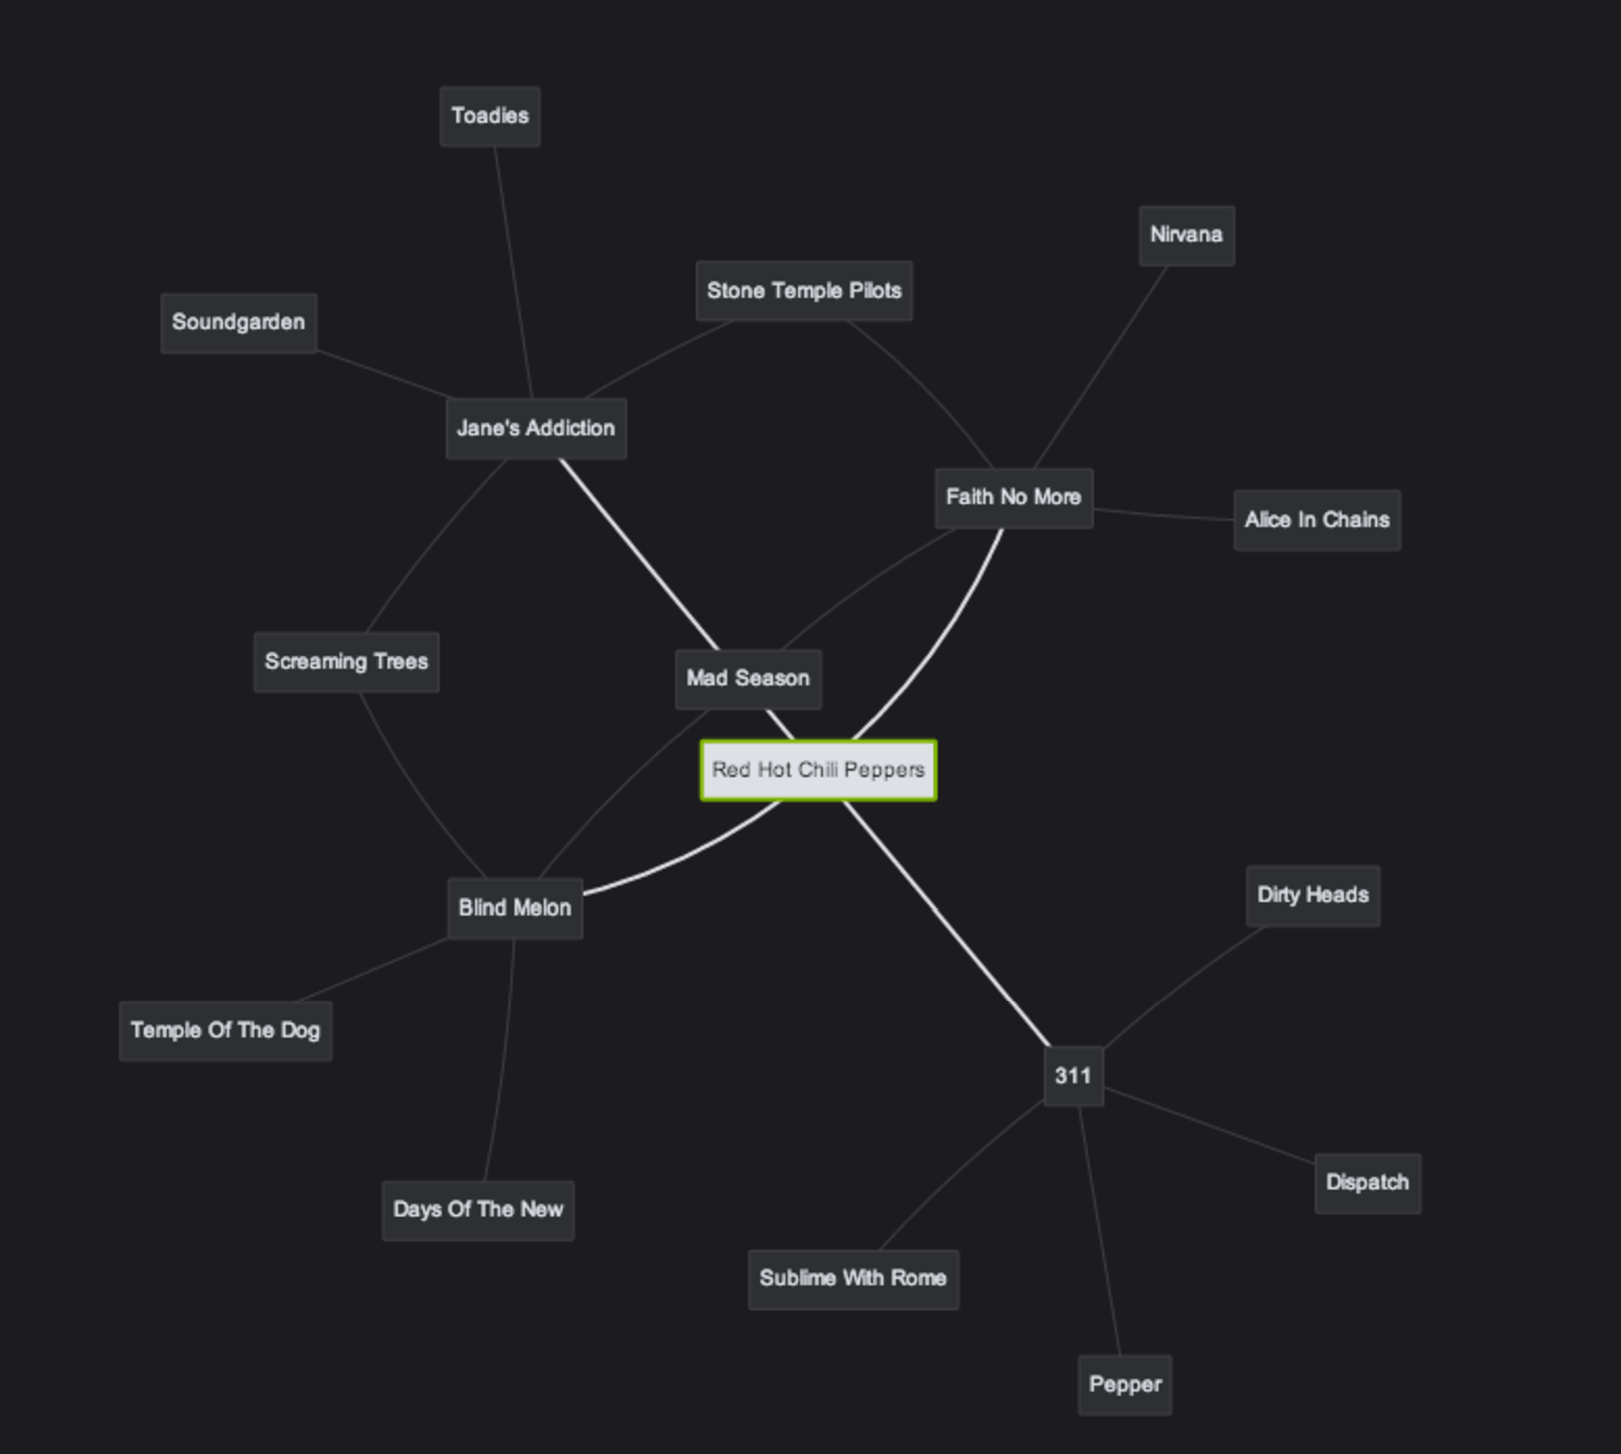
\includegraphics[width=\textwidth]{map_creation_notreemode.pdf}
        \end{center}
        \caption{Graph created with all the connections with "Red Hot Chilli Peppers" as the root node.}
        \label{fig:graph_notreemode}
      \end{figure}

      \hfill \\
      \indent \emph{
      From now on, if the graph is a tree, it will be said that the algorithm is using the \emph{Tree Mode}.
      So the example \ref{fig:graph_treemode} is a \emph{Tree Mode} example, and the examples \ref{fig:graph_notreemode} and \ref{fig:graph_notreemode2} are not \emph{Tree Mode} examples\footnote{
        Note that, sometimes, even if the algorithm is not on tree mode, it might generate a tree, simply because there were no missing edges between the nodes to be added to the graph.
      }.}
      \hfill \\

      Note (\ref{fig:graph_notreemode}) how "Stone Temple Pilots" is now a child of both "Faith No More" and "Jane's Addiction".
      Also note that the same behaviour is visible with the nodes "Mad Season" and "Screaming Trees".

      At this point, the user's perception of the artist "Stone Temple Pilots" is now different from the previous example (Figure~\ref{fig:graph_treemode}).
      These added connections are, in a way, clustering together the most connected nodes.
      In this particular example, one could see an improvement with this approach: it contributes to the user's perception of the artist's network by making sure the user knows that those specific artists are more connected between them, than any others.
      The fact is that only three extra edges where added, meaning there is not much visual clutter in the visualization. \\

      However, that might not always be the case.

      One could argue that the "Mad Season" artist node is already disturbing the visual representation by being drawn over an edge.

      In fact, with the exact same values of branching, depth and tree mode off, when creating a graph for the artist "Mariza", the visual clutter is so strong that the graph becomes confusing and not very helpful: Figure~\ref{fig:graph_notreemode2}.

      \begin{figure}[tb]
        \begin{center}
          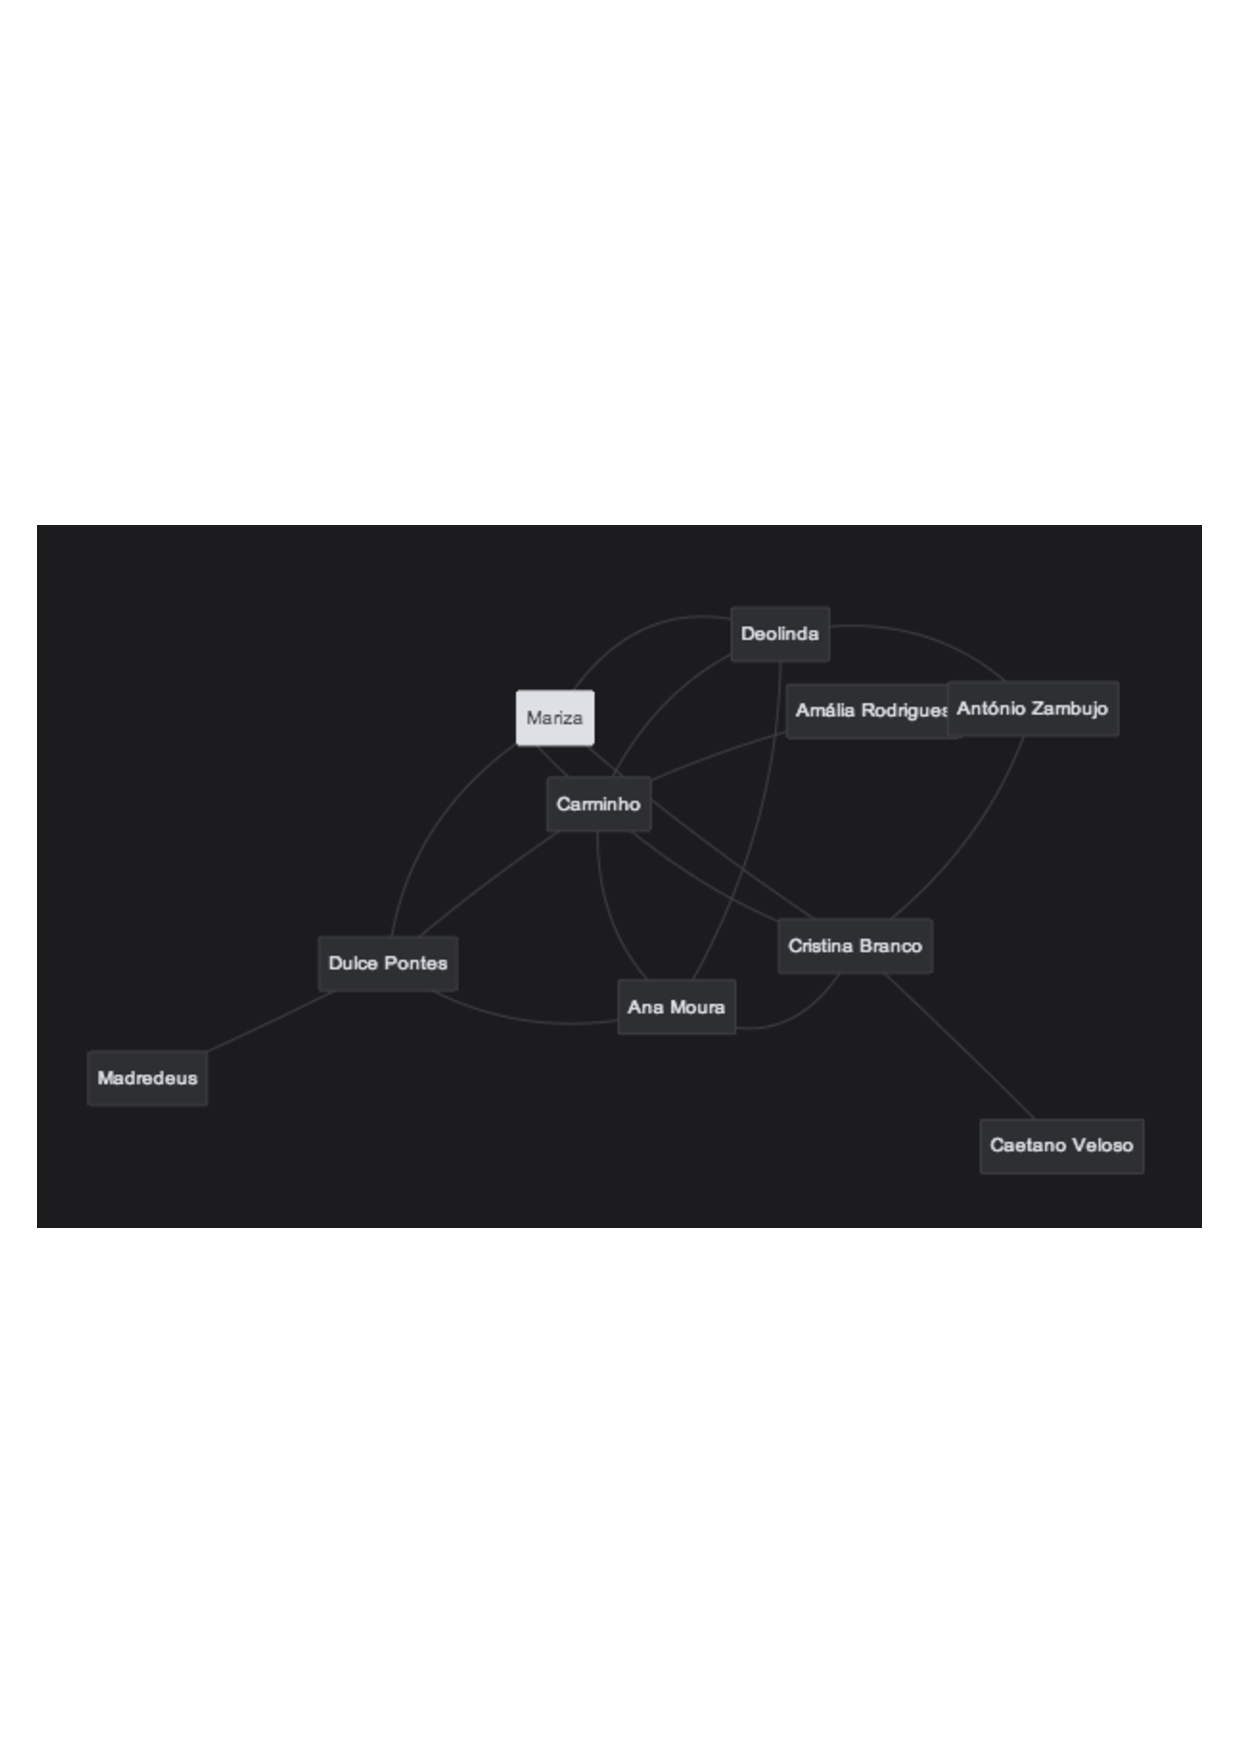
\includegraphics[width=\textwidth]{graph_notreemode2.pdf}
        \end{center}
        \caption{Graph created with all the connections with "Mariza" as the root node.}
        \label{fig:graph_notreemode2}
      \end{figure}

      The cluster of nodes in the center makes it clear that those specific nodes are really connected between them. 
      But then, the edges, that are forcing those nodes together, are creating a visual clutter that might not be so desirable.
      Instead of creating a visual map of the artists' network for the user to perceive, explore and change in its own way, the representation is more contained, static and not so visually appealing.
      \hfill \\

      So on one hand, the \emph{clustering} of the nodes seems like an interesting feature.
      It allows for a much more in-depth user access to the underlining information of the related artists.
      But on the other hand, the focus of the visualization (to show a map of the artists' network) is shifting to this cluster-like representation.

      Both perspectives are advantageous depending on the data they are operating on (as seen in the previous examples).
      So instead of choosing only one method, both were chosen: by default, the graph creation algorithm is on tree mode, and the user can turn it off from a settings menu.
      This allows for the user to choose the visual representation method that suits its needs.

      \paragraph{Depth and Branching values} \hfill \\
      The depth and branching values have been mentioned before in this chapter, but not further explained.

      The \textbf{depth} value of a graph determines how deep the recursive algorithm is.
      The previously presented example (\ref{fig:graph_treemode}) has a depth value of 2.
      The example \ref{fig:graph_depth3} has a depth value of 3.

      \begin{figure}[hb]
        \begin{center}
          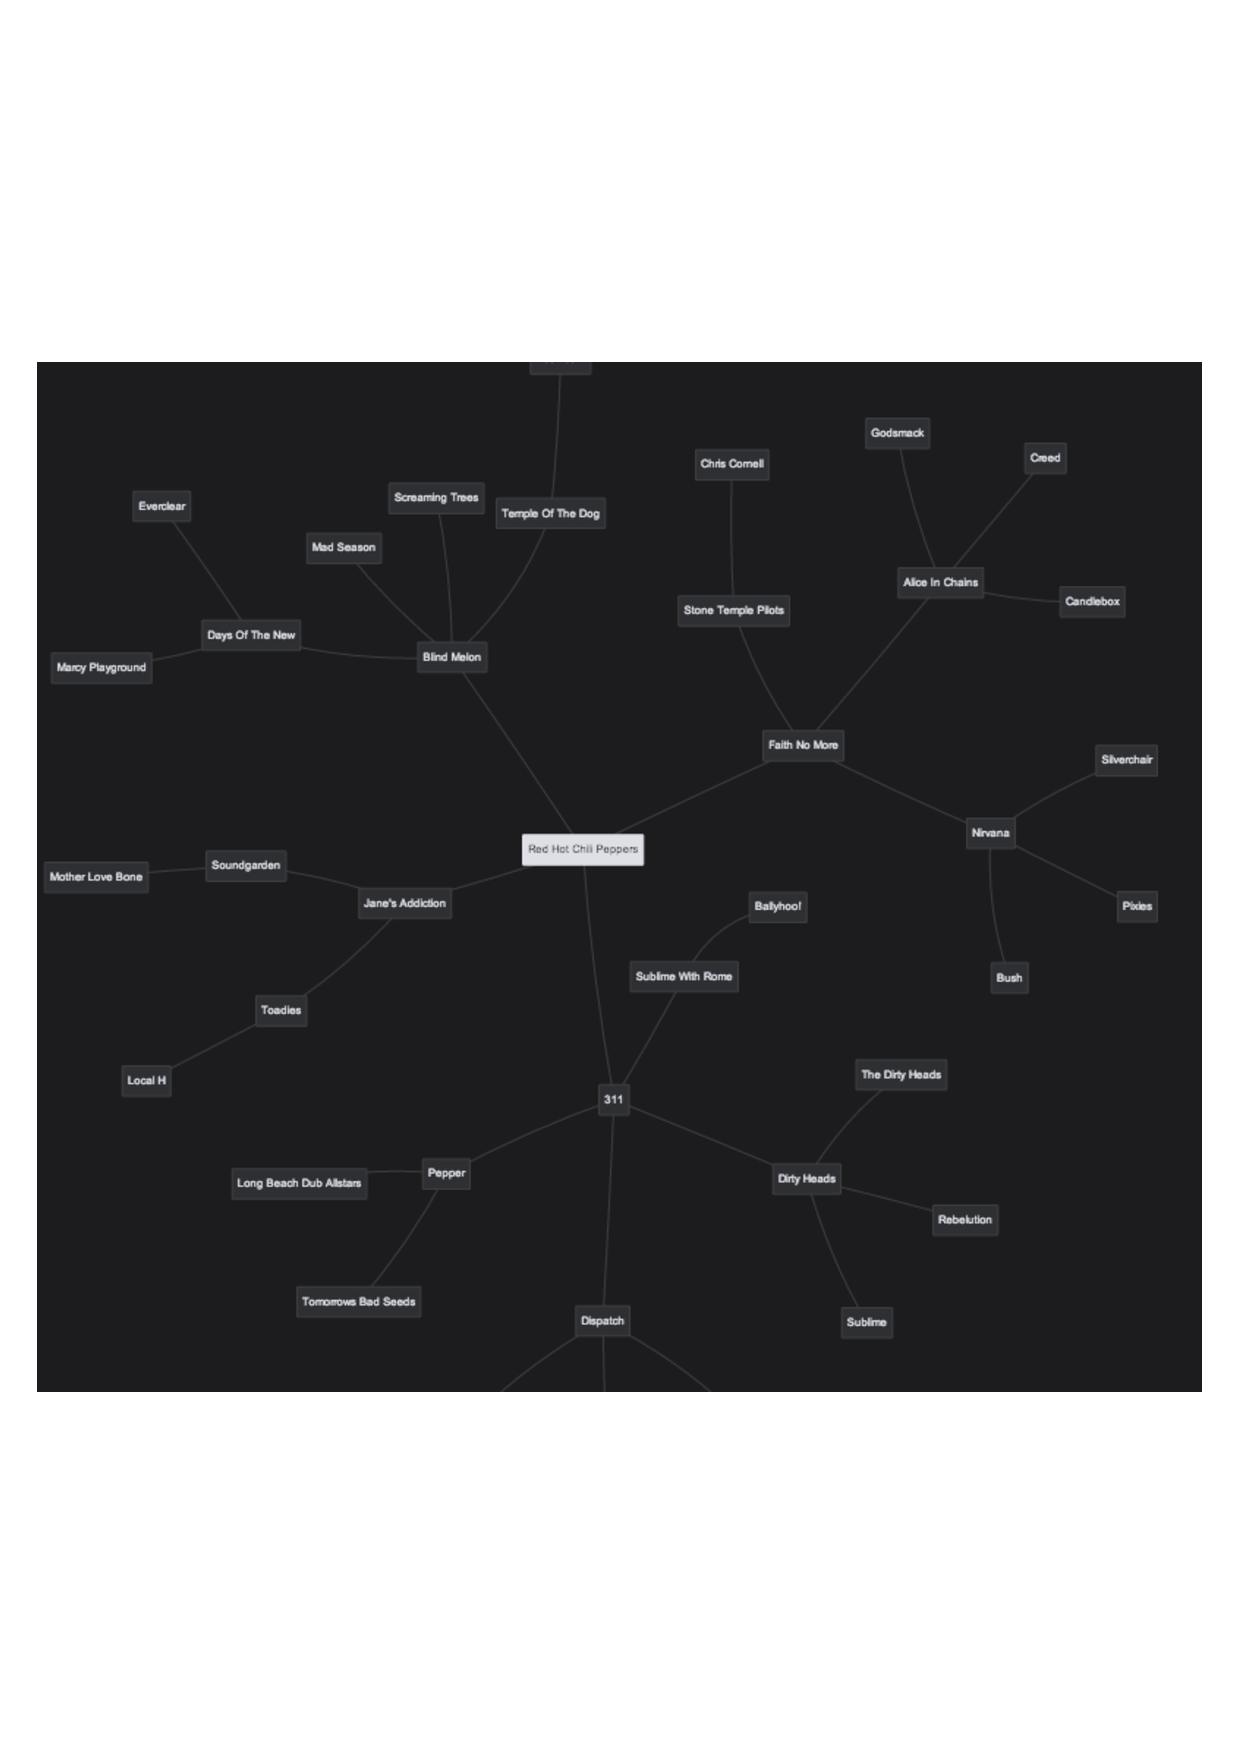
\includegraphics[width=\textwidth]{graph_depth3.pdf}
        \end{center}
        \caption{Graph with depth value of 3}
        \label{fig:graph_depth3}
      \end{figure}
      In short, depth is the maximum distance between the root node and any other node in the graph.

      The \textbf{branching} value of a tree graph determines the maximum number of child nodes a node can have.
      The example \ref{fig:graph_treemode} has 4 branching.

    % subsubsection visualization (end)

    \subsubsection{Visualization Parameters} % (fold)
    \label{ssub:visualization_parameters}
    
    The visualization parameters are the branching and depth values, as well as the option to enable/disable the tree mode.

    To allow the user to change these values, a settings menu was added to the application, and can be seen in Figure~\ref{fig:settings_menu}.
    When the user changes the parameters, the graph refreshes accordingly.

    \begin{figure}
      \begin{center}
        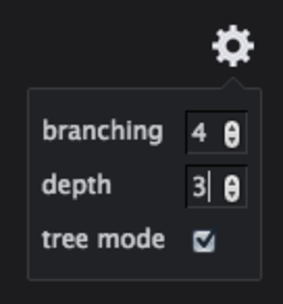
\includegraphics[width=0.8\textwidth]{settings_menu.pdf}
      \end{center}
      \caption{The settings menu that allows the user to change the visualization parameters.}
      \label{fig:settings_menu} 
    \end{figure}

    % subsubsection visualization_parameters (end)

    \subsubsection{Graph Edition} % (fold)
      \label{ssub:edition}

      The available features to edit the graph are as follow: expand node, delete node and create a new map.
      These interactions are available in the Artist Menu (\ref{ssub:artist_info}).

      \paragraph{Expand node} \hfill \\
      This option allows the user to expand a node further (ignoring the graph's branching value).
      Given the previous example \ref{fig:graph_treemode}, if the "Dispatch" node gets expanded, it results in \ref{fig:node_expanded}.

      To put it simply, to expand a node, one performs one iteration of the graph creation algorithm.

      \begin{figure}[tb]
         \begin{center}
           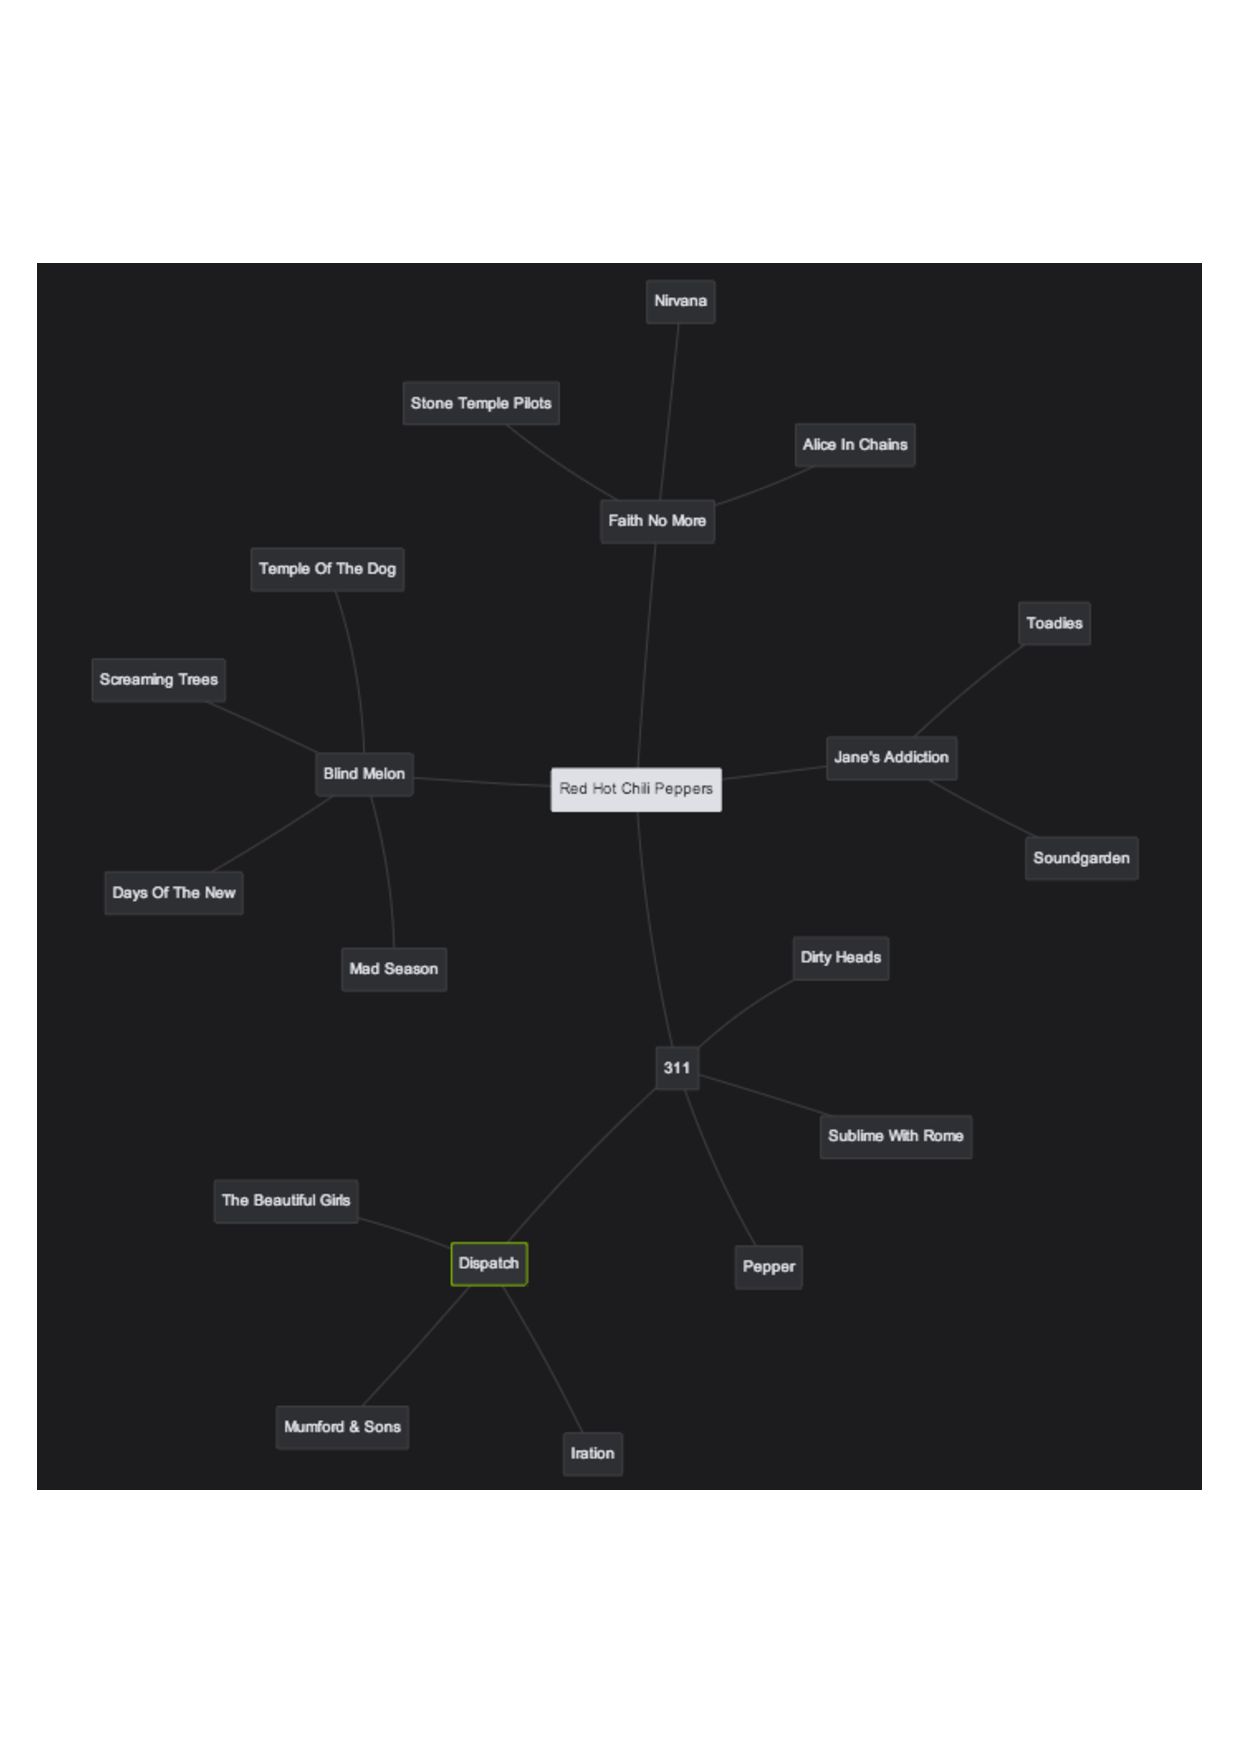
\includegraphics[width=\textwidth]{node_expanded.pdf}
         \end{center}
         \caption{"Dispatch" artist node expanded.}
         \label{fig:node_expanded}
      \end{figure}

      \paragraph{Delete node} \hfill \\
      This options allows the user to delete a node from the graph.
      Useful for when the user wants to construct the graph to its needs.

      \paragraph{New map} \hfill \\
      The user may choose to create a whole new graph from a another node.
      This way the root node will be the selected node.


    % subsubsection edition (end)

    \subsubsection{Artist Info} % (fold)
      \label{ssub:artist_info}
      The user is able to see additional information about artists in the Artist Menu (\ref{fig:artist_menu}) such as its popularity value, albums and tags, as well as perform the \emph{expand} and \emph{new map} functions described in \ref{ssub:edition}.

      \begin{figure}[tb]
        \begin{center}
          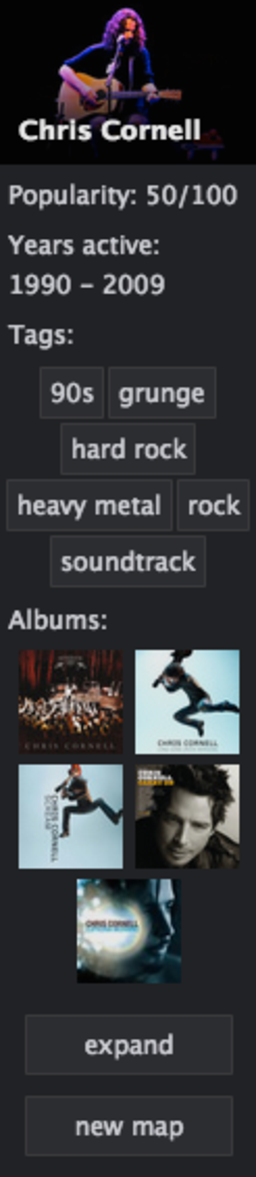
\includegraphics[width=\textwidth]{artist_menu.pdf}
        \end{center}
        \caption{Artist Menu with information about "Chris Cornell"}
        \label{fig:artist_menu}
      \end{figure}

      When the user selects a node by clicking on it, the artist menu updates the displayed information.

      The \emph{popularity} and the \emph{albums} are metadata information retrieved from Spotify's API framework (\ref{sub:spotify_apps}).
      The tags, however, are not supported by Spotify's API.
      For that, Echonest's API was used.

      \paragraph{Echonest's Terms} \hfill \\
      Echonest's tags are very similar to the most commonly known \emph{music genres} (like jazz, country, rock), but they also might include more alternative descriptive terms (progressive metal, symphonic, soundtrack).

      The connection between the two APIs is possible thanks to the Project Rosetta Stone\footnote{\url{http://developer.echonest.com/docs/v4\#project-rosetta-stone}}.
      For example, to retrieve the terms\footnote{Echonest calls it terms. From now on, terms and tags will be used interchangeably} of an artist from Echonest's metadata API using the Spotify's Artist ID, the following query is used: \\

      \url{
        http://developer.echonest.com/api/v4/artist/terms?api_key=API_KEY&format=json&sort=weight&id=spotify-WW:artist:65nZq8l5VZRG4X445F5kmN
      } \\

      The \emph{id} parameter is similar to the Spotify's URI scheme (\ref{sub:metadata_api}), and this allows for retrieving extra information about the artist that Spotify's API does not provide.

      \emph{Sort} is another interesting parameter. 
      In general, artists have more than 10 or 15 terms.
      Each term has a value of \emph{frequency} and a value of \emph{weight}, and both are float values that range between zero and one.
      No official documentation was found to explain what do these values represent, but Paul Lamere\footnote{Paul Lamere is Director of Developer Platform at \url{the.echonest.com} (\url{http://the.echonest.com/company}). Also blogs here: \url{http://musicmachinery.com}} explains\footnote{thread in the forum for Echonest's API users - \url{http://developer.echonest.com/forums/thread/353}} that:

      \begin{quote}
      \emph{
        term frequency is directly proportional to how often that term is used to describe that artist
      }
      \end{quote}

      \begin{quote}
      \emph{
        term weight is a measure of how important that term is in describing the artist
      }
      \end{quote}

      So given this, one can conclude that by sorting the terms of an artist by its frequency value, the top terms will be more general (rock, pop, jazz) and not very descriptive or specific of an artist.
      And by sorting the tags by weight, one will get the most descriptive tags of that specific artist.

      Clearly, in this case, for the Artist Menu the weight parameter is very helpful, and so, the sort parameter used for the query is \emph{weight}.
      As seen in \ref{fig:artist_menu}, the tags shown are very descriptive of the artist (grunge, 80s, hard rock). \\

    % subsubsection artist_info (end)

    \subsubsection{Tags Overlay} % (fold)
      \label{ssub:tags_overlay}

      The tags overlay menu (\ref{fig:tags_overlay}) is meant to enhance the user's perception on the displayed artists' nodes regarding their tags.

      \begin{figure}[tb]
        \begin{center}
          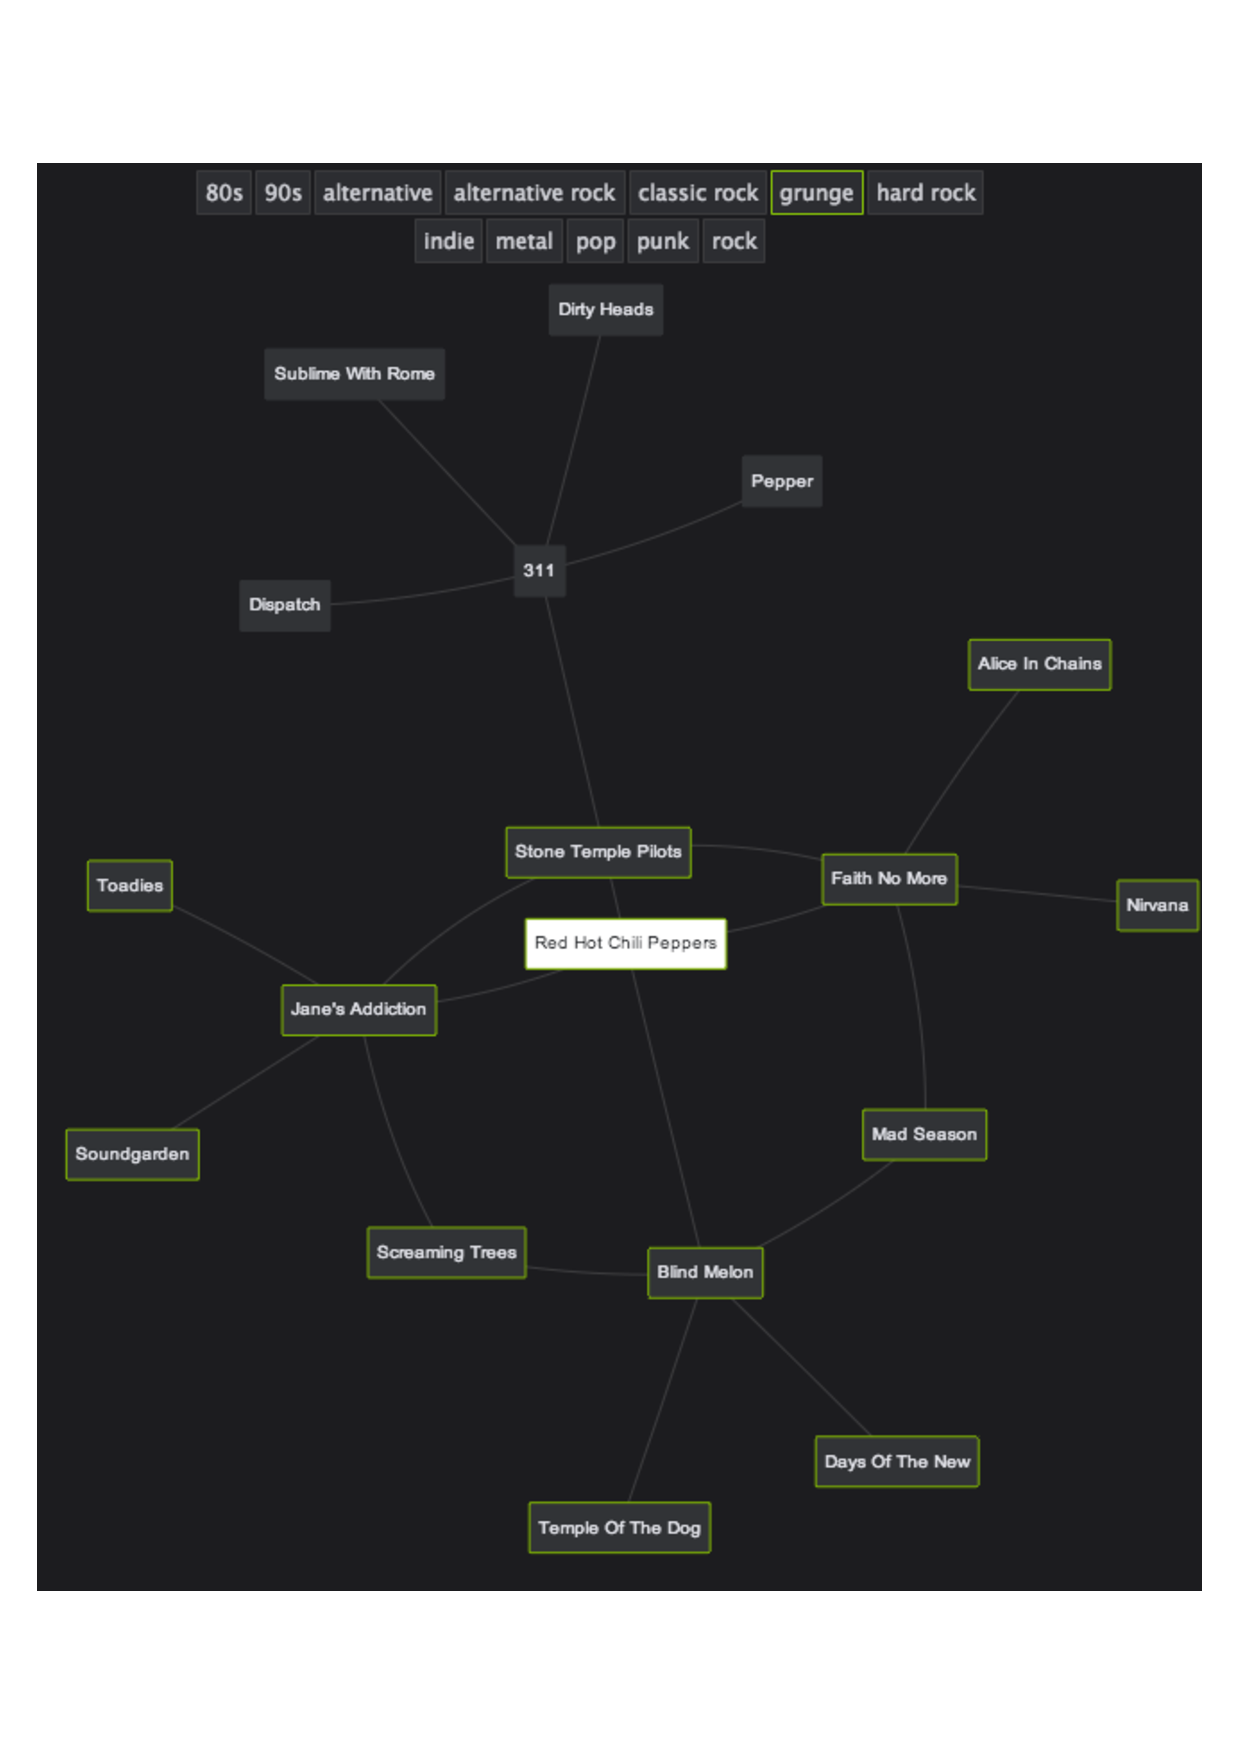
\includegraphics[width=\textwidth]{tags_overlay.pdf}
        \end{center}
        \caption{Tags overlay for the displayed graph. When the tag "grunge" is selected the corresponding artist nodes are selected}
        \label{fig:tags_overlay}
      \end{figure}

      These tags are the same ones used in the Artist Menu (\ref{fig:artist_menu}).

      The tags are selectable, and so, when clicked, the respective artist nodes that are described by those tags, are highlighted (as seen in Figure~\ref{fig:tags_overlay}).

      The tags shown in this menu, are just a small sample of the artists' tags of the whole graph.
      For example, for the graph in the Figure~\ref{fig:graph_anamanaguchi}, the total count of unique tags in the whole graph is 93.
      To select which tags to show, those same 93 tags were sorted by frequency in the graph, and then the top 12 ones are shown.

      This way, the tags in the overlay are significant for the graph, by helping the user to visually group together some related artists.

      \begin{figure}
        \begin{center}
          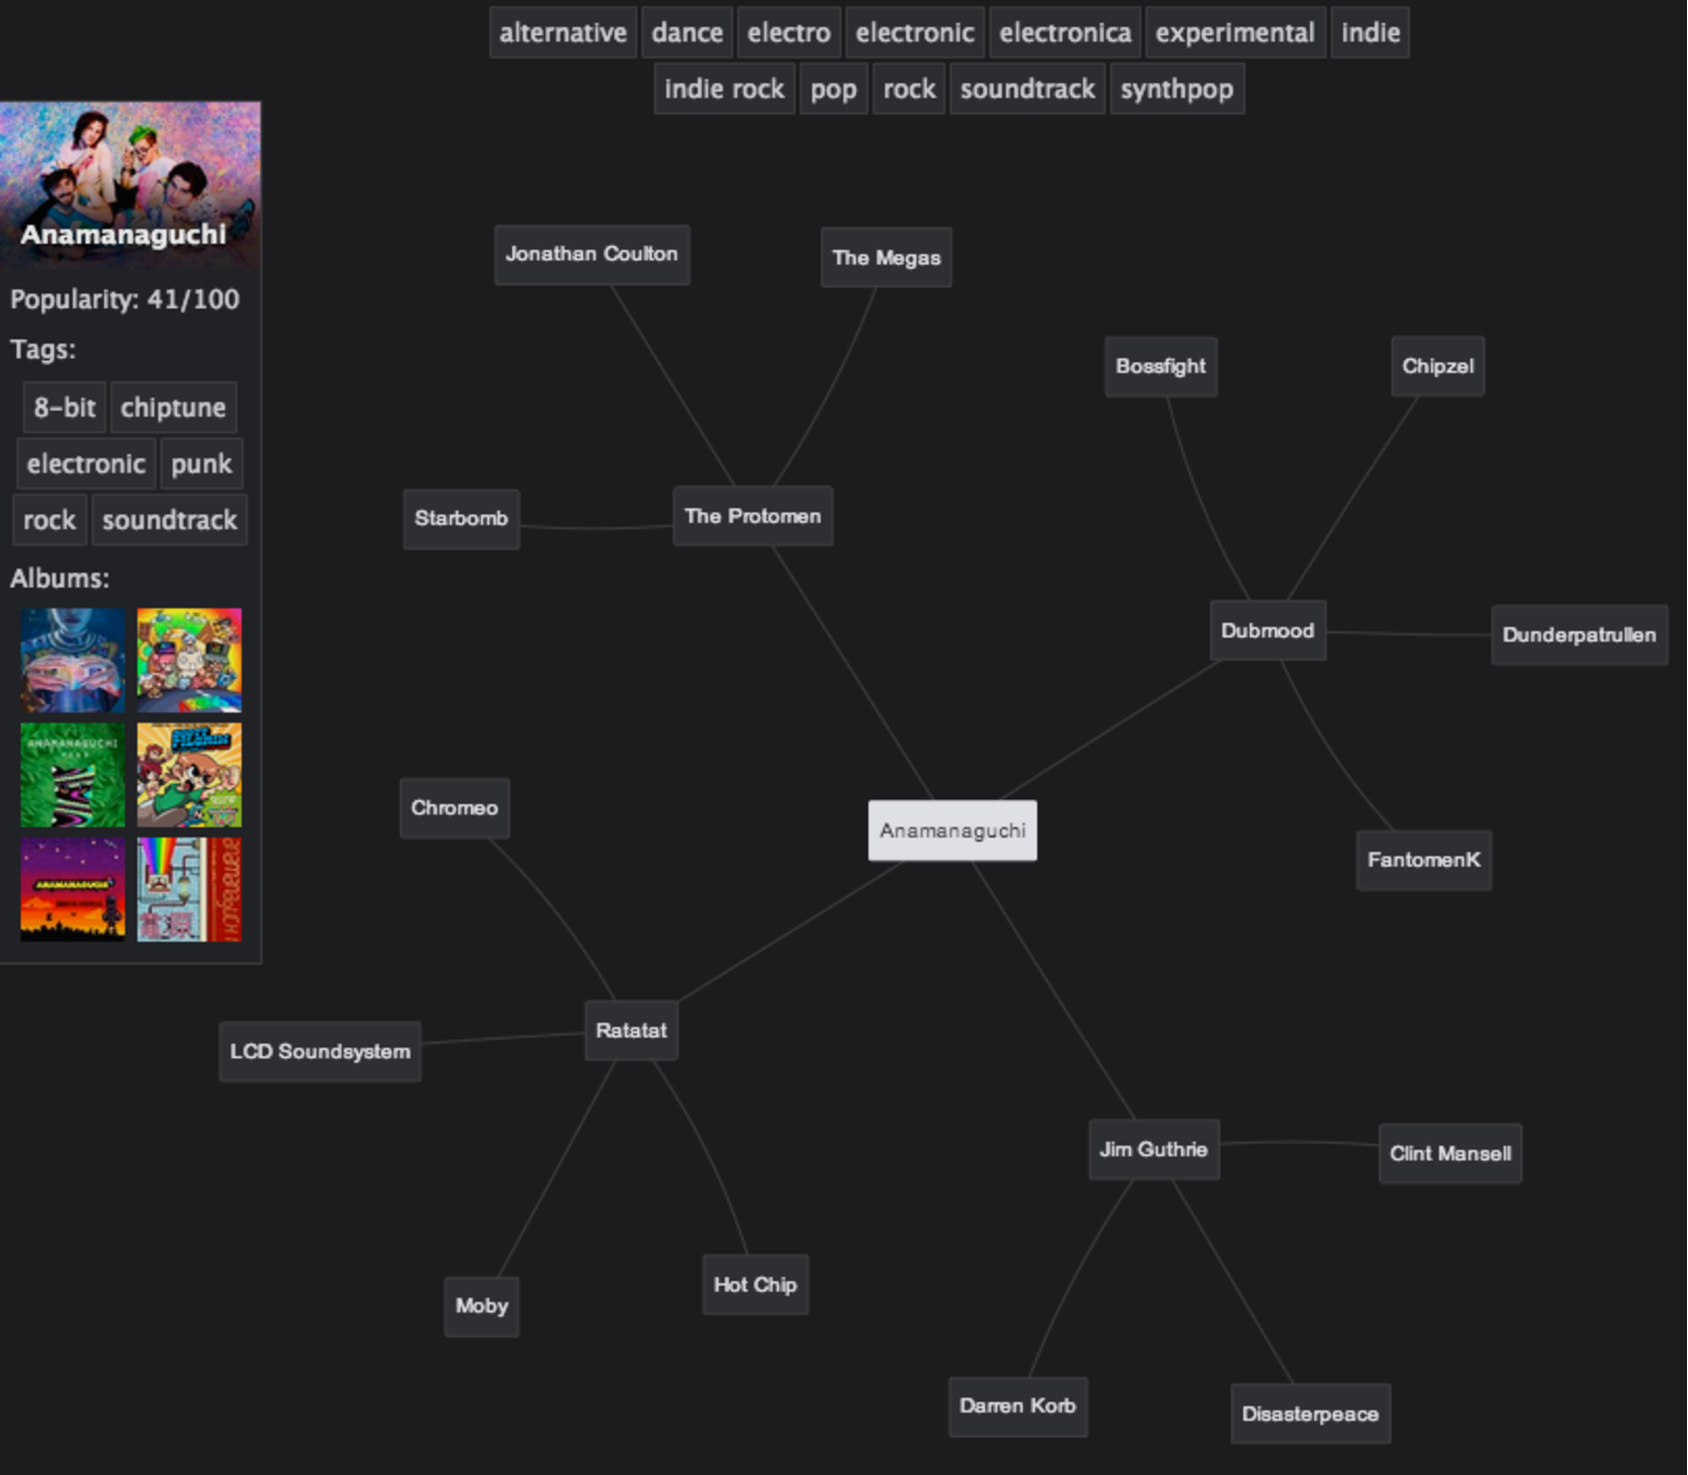
\includegraphics[width=\textwidth]{graph_anamanaguchi.pdf}
        \end{center}
        \caption{Graph for "Anamanaguchi". The tags shown above are only but a small sample of all the tags of all the artists in the graph}
        \label{fig:graph_anamanaguchi}
      \end{figure}

    % subsubsection tags_overlay (end)

  % subsection main_features (end)


  \subsection{Development Processes} % (fold)
    \label{sub:development_process}

    The primal objectives for the RAMA Spotify Application were to implement the basic functionalities that RAMA's website\footnote{\url{http://rama.inescporto.pt/app}} offers.

    Incrementally, they were implemented, tested and added to the application.
    A timeline (chronological order from bottom to top) with the added features (each update release) can be seen in \\ 
    \indent \url{https://github.com/carsy/rama-spotify/releases} \\

    An overview of pushed commits can be viewed in Figure~\ref{fig:code_contributions}.

    \begin{figure}
      \begin{center}
        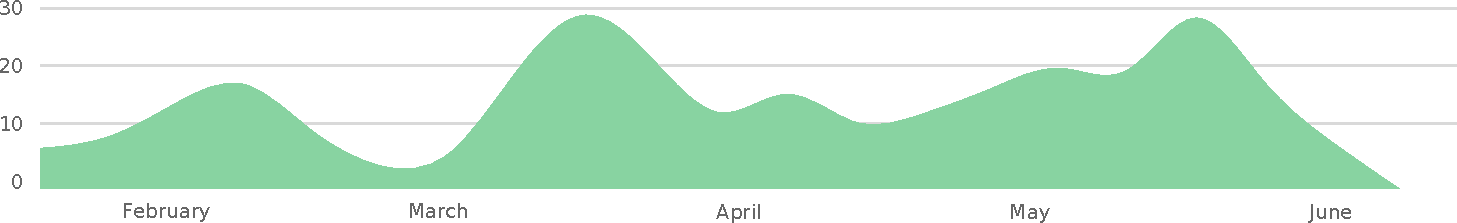
\includegraphics[width=\textwidth]{code_contributions.pdf}
      \end{center}
      \caption{Graph showing the number of commits to the project from January to June, 2014. All of the development code was hosted in \url{Github.com}. Adapted from \url{https://github.com/carsy/rama-spotify/graphs/contributors}}
      \label{fig:code_contributions}
    \end{figure}

    Unit tests were added for each feature.
    The tests were run locally to ensure that previous features were still working during development.
    Also to ensure that every release had the tests passing, the project was integrated in Travis's Continuous Integration\footnote{Travis: \url{http://travis-ci.org}} system: \\
    \indent \url{http://travis-ci.org/carsy/rama-spotify}.

    This way, after every push of a new release, the project gets build and the unit tests run automatically. \\

    The solution was also submitted to validation several times during its development.
    After each release, a constant small group of alfa-testers (3 people) reviewed the state of the application.
    Their feedback would be carried over the next release: bug fixes, improvements, etc.
    This was the testing cycle that allowed to validate the implemented features.
    This iterative process was managed using the issue tracking system of Github\footnote{Github: \url{http://github.com}}: \url{https://github.com/carsy/rama-spotify/issues}.
    Given this iterative process of implementation and feedback, the solution would be better prepared for future occasional beta-testing.
    
    % TODO compare with the previous work plan

  % subsection development_processes (end)

% section prototype (end)

  \clearpage

\section{Validation} % (fold)
\label{sec:validation}

  In order to validate the proposed method, user tests were done with Spotify users and non-Spotify Users.
  They represent the second group of testers and will be referred as the beta-testers.

  \subsection{User Tests} % (fold)
  \label{sub:user_tests}

    The proposed application is targeted at Spotify Users.
    However, non-Spotify users also tested RAMA's Spotify Application after a few moments of using Spotify's interface.

    During the test, the user was asked to first use Spotify only.
    The task was to find a couple of new artists that the user liked.
    This first task should take no more than 7 minutes, depending on the user.

    Next, the user was asked to open the RAMA application and do the same (no more than 7 minutes as well).
    Given this, the user is forced to compare the two approaches: discovering new music with Spotify only, and discovering new music with RAMA's Spotify Application.

    After the test, the user filled a short inquiry about the experiment, which contained the following questions:

    \begin{enumerate}
      \item Are you a Spotify user?
      \item Did the RAMA application help you discover new interesting artists?
      \item Do you think you would use the application to discover new music?
      \item Was the application well integrated with Spotify?
    \end{enumerate}

  % subsection user_tests (end)


  \subsection{Data Analysis} % (fold)
  \label{sub:data_analysis}

    A total of 15 beta-testers participated in the experiment.

    \subsubsection{Question 1: Are you a Spotify user?} % (fold)
    \label{ssub:question_1}

      This question was meant to establish the user's experience with Spotify.

      The results can be seen in Table~\ref{tab:question1}.

      \begin{table}[hb]
         \begin{center}
           \begin{tabular}{l|c}
       
           \hline
           \textbf{Answer} & \textbf{Nº of responses} \\
           \hline

           \hline
              Yes, I use it as my main way to listen to music & 3 \\
              Yes, I use it from time to time & 3 \\
              No, but I have used/tried it at least once & 4 \\
              No, this is my first time using it & 5 \\
           \hline
           \end{tabular}
         \end{center}
         \caption{Results for question 1.}
         \label{tab:question1}
       \end{table}

       This test group is relatively well distributed with 6 Spotify Users, and 9 non-spotify users.
    
    \subsubsection{Question 2: Did the RAMA application help you discover new interesting artists?}
    \label{ssub:question_2}

      This was a yes or no question: 14 responded "yes", whereas, 1 responded "no".

      It is clear that RAMA's Spotify Application did not faulted the initial purpose of letting the user discover new music.


    \subsubsection{Question 3: Do you think you would use the application to discover new music?}
    \label{ssub:question_3}

    This is the ultimate question that leaves the user thinking if RAMA in fact a usable way of discovering new music within Spotify.

      \begin{table}[hb]
         \begin{center}
           \begin{tabular}{l|c}
       
           \hline
           \textbf{Answer} & \textbf{Nº of responses} \\
           \hline

           \hline
            Yes, this is what Spotify is missing! & 5 \\
            Yes, sometimes it's nice to see this visual representation & 10 \\
            No, it does not add much to Spotify & 0 \\
            No, I wouldn't use it. I like Spotify the way it is & 0 \\
           \hline
           \end{tabular}
         \end{center}
         \caption{Results for question 3.}
         \label{tab:question3}
       \end{table}

      The results indicate that the visual representation is indeed a very useful feature when discovering new music.

      \subsubsection{Question 4: Was the application well integrated with Spotify?}
      \label{ssub:question_4}

        In a scale of 1 to 5, given 1 to be "I felt the app was out of place" and 5 to be "I felt the app was part of Spotify", the users were asked to grade the application's integration into Spotify.

        \begin{table}[hb]
           \begin{center}
             \begin{tabular}{c|c}
         
             \hline
             \textbf{Answer} & \textbf{Nº of responses} \\
             \hline
             1 & 0 \\
             2 & 0 \\
             3 & 1 \\
             4 & 4 \\
             5 & 10 \\
             \hline
             \end{tabular}
           \end{center}
           \caption{Results for question 4.}
           \label{tab:question4}
         \end{table}

         The majority of the users felt that the application was part of Spotify.
         This is a very important result which indicates that the developed prototype blends very well with Spotify's Desktop Client.
  
  % subsection data_analysis (end)
% section validation (end)


\section{Summary} % (fold)

  The used tools during the whole development process proved to be very useful.
  All of the proposed features for the prototype were implemented within schedule, and the feedback from the users was very positive.


% section summary (end)